\documentclass{article}
\title{ECE 478-- Homework 2}
\usepackage{graphicx}
\usepackage{fancyhdr}
\usepackage{enumitem}
\usepackage{amsmath}
\usepackage{float}
\setlist[enumerate, 1]{label=\thesection.\arabic*}
\usepackage{amsmath}
\pagestyle{fancy}
\fancyhf{}
\fancyhead[L]{Gianni Avilan-Losee}
\fancyhead[C]{ECE 478}
\fancyhead[R]{Homework 2}
\fancyfoot[C]{\thepage}
\usepackage{microtype}
\usepackage{textcomp, gensymb}
\author{Gianni Avilan-Losee}
\setcounter{section}{2}
\begin{document}
\begin{enumerate}
	\item For an nMOS transistor, its I-V characteristics may be described by the first-order Shockley model, \[
		I_{ds} = \begin{cases}
			0 & V_{gs} < V_t \\
			\beta(V_{GT} - \frac{V_{ds}}{2})V_{ds} & V_{ds} < V_{dsat}\\
			\frac{\beta}{2}V^2_{GT} & V_{ds} > V_{dsat}\\
		\end{cases},
	\]	
	for the cutoff, linear, and saturation regions of operation, respectively. \(\beta\) is given by \[
		\beta = \mu_n C_{ox} \frac{W}{L},
	\]
	where \(\mu_n\) is electron mobility, \(C_{ox}\) is gate oxide capacitance per unit area, and \(W\) and \(L\) refer to the width and length of the transistor channel, respectively.

	Plotting the I-V curve, using the piecewise function given above, for an nMOS transistor with a \(\frac{W}{L}\) ratio of \(\frac{4}{2}\), a gate oxide thickness of \(100\)\r{A} (used to calculate \(C_{ox}\)), a threshold voltage of \(0.7\)V, and an electron mobility of \(350 \frac{cm^2}{V \cdot s}\) for \(V_{gs} = 0, 1, 2, 3, 4,\) and \(5\)V,
	\begin{figure}[H]
	  \centering
	  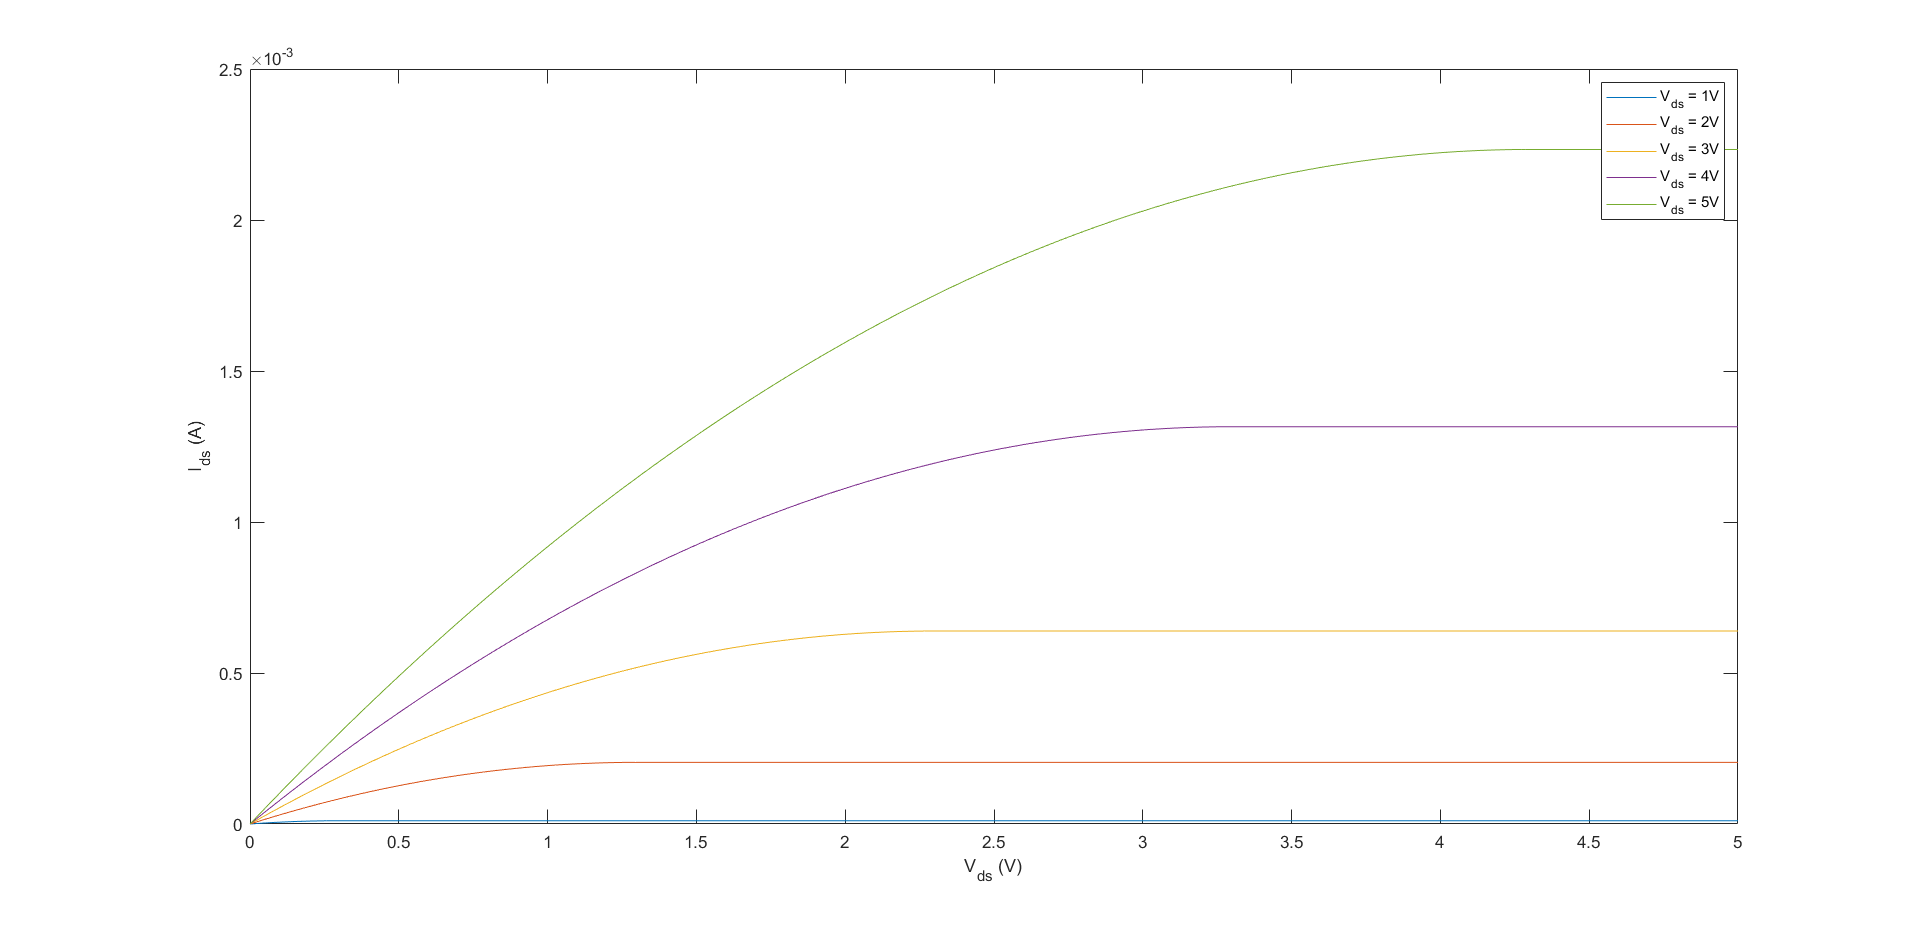
\includegraphics[width=1\textwidth]{figures/homework_2-fig_1.png}
		\caption{I-V curve for various values of \(V_{gs}\)}
	  \label{fig:I-V Curve}
	\end{figure}
	Note that at \(V_{gs} = 0\text{V}\), the transistor is in cutoff mode, and no current flows between source and drain.
\setcounter{enumi}{3}
\item To find gate capacitance per micron of width \(C_{permicron}\), we may use the formula for gate capacitance per unit area, \(C_{g} = C_{ox}WL\). Dividing out the width of the gate leaves \[
		\frac{C_{g}}{W} = C_{permicron} = C_{ox}L = 0.194\frac{\micro\text{F}}{\micro\text{m}}.
\]
\setcounter{enumi}{8}
\item The threshold voltage of any MOS transistor is defined as the minimum gate-to-source voltage \(V_{gs}\) that generates an inversion layer at the boundary between the insulating dielectric layer and the MOS transistor's body. In an nMOS transistor, the body is generally constructed with a p-type substrate (hence the "inversion" layer that forms as negatively charged particles are drawn to the body-dielectric boundary). The device's source and drain terminals, on the other hand, are constructed with an n-type material. 

 Thus, \(V_{gs}\) in an nMOS must be positive to generate a channel for current to flow between source and drain. The effect of raising the electrical potential of the body relative to ground would be to increase the threshold voltage, since a higher voltage relative to ground would now need to be provided to the gate to generate a conducting channel. 

 Conversely, lowering the electrical potential of the body relative to ground would have the opposite effect, decreasing the threshold voltage needed to generate a conducting channel. 
 \setcounter{enumi}{19}
 \item
	 \begin{figure}[H]
	   \centering
		 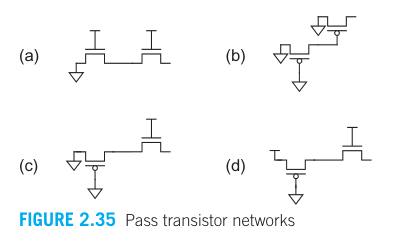
\includegraphics[width=0.6\textwidth]{figures/homework_2-fig_2.png}
	   \caption{Pass transistor networks}
	   \label{fig:Textbook graphic}
	 \end{figure}
 \begin{enumerate}[label=\alph*)]
	 \item The gate of both series-connected nMOS transistors are tied to \(V_{DD}\), while the drain of the first is tied to ground. At the source of the second transistor, we may define the output voltage as \(V_{s} = 0\text{V}\), since the gate-to-source voltage \(V_{gs}\) will remain well above \(V_{tn}\) when the source of both nMOS devices is pulled to ground.
	 \item Assuming both pMOS transistors share the same threshold voltage \(V_{tp}\), the first transistor will provide a degraded voltage \(|V_{tp}|\) to the second transistor's gate. Then, the second pass transistor will degrade the output by the same threshold drop, leaving a total output voltage of \(V_{s} = 2|V_{tp}|\). 
	 \item The inital pMOS pass transistor will pass a degraded voltage to the drain of the series-connected nMOS transistor, which will pass a "strong" voltage to its source terminal, resulting in a total output voltage of \(V_{d} = V_{s} = |V_{tp}|.\) 
		\item In this configuration, the initial pMOS device passes a "strong" 1 to the drain of the nMOS device, which passes a degrade output voltage of \(V_{DD} - V_{tn}\).
	\end{enumerate}
\item 
	\begin{enumerate}[label=\alph*)]
		\item Given an input voltage \(V_{in} = 0\text{V}\), the nMOS transistor, in its "on" state, will pass \(0\text{V}\) to the source, resulting in a gate-to-source voltage \(V_{gs} = 1.2\text{V}\). Since \(V_{gs} > V_{tn}\), the output will not be degraded and \(V_{s} = 0\text{V}\). This agrees with our notion that nMOS transistors pass a "strong" 0. 
		\item Given \(V_{in} = 0.6\text{V}\), \(V_{gs}\) will drop to \(0.6\text{V}\). Since \(V_{gs}\) is still greater than \(V_{tn}\), the  output will not be degraded, and \(V_{s} = 0.6\text{V}\). 
		\item At \(V_{in} = 0.9\), \(V_{gs}\) drops to \(0.3\text{V}\), below the threshold voltage. Now, the output voltage is degraded, and \(V_{s} = V_{DD} - V_{tn} = 0.8\text{V}\), a degraded 1.
		\item In this case, \(V_{in}\) is still greater than \(V_{tn}\), and so the output remains at a degraded 1, with \(V_{s} = 0.8\text{V}\).
	\end{enumerate}
\end{enumerate}
\end{document}
